\section{Experimental methods and apparatus}\label{sec:experimental-technique-and-apparatus}
To examine the diffraction pattern from different slit patterns (and eventually a helix) we use the system described in Figure~\ref{fig:Apparatus}.
\begin{figure}[H]
    \centering
    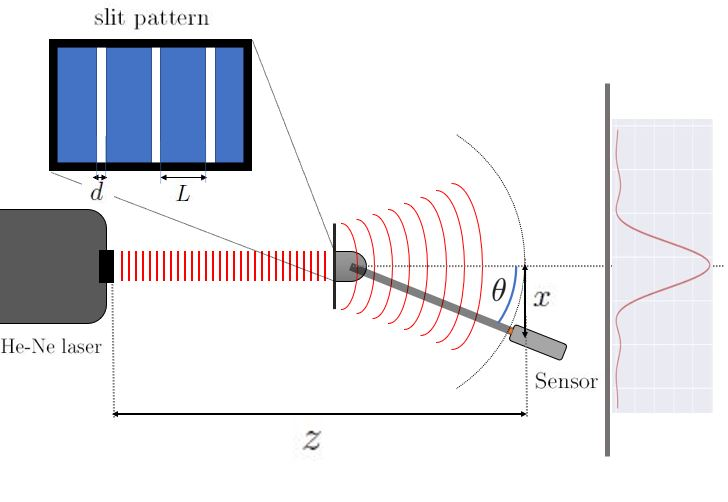
\includegraphics[width=0.9\columnwidth]{figures/Apparatus.JPG}
    \caption{A description of the system used to measure the intensity of light coming from a He-Ne laser at different angles. An example of a slit
    pattern is shown, but can be swapped for any diffracting object}
    \label{fig:Apparatus}
\end{figure}
Where the He-Ne laser produces an approximately monochromatic plane wave with $\lambda=632.8 [nm]$ and our sensor is at a fixed distance from the slits with $z=0.855 [m]$.
The angle $\theta$ and the Intensity $I$ were measured using a resistor and a photodiod, the voltage on these resistors ($V\propto\theta,I$) was
measured at a rate of $40[Hz]$ and a resolution of $\Delta V\approx10^{-3}[V]$.
Prior to every measurement we align the laser beam with the sensor by detecting the point of maximum intensity, then place the slits perpendicular to
the beam.
The slits are then moved along the x axis until we measure maximum amplitude for a single slits and n slits, or between the two maxima for double slit patterns.
These procedures are key to make sure our wave is a good approximation for a plain wave and it is reaching the slits with uniform phase thus avoiding major differences from our models' assumptions.
The sensor was then moved to scan the intensities at some range of angles which were then converted to distances on our theoretical screen.
We also note that the sensor has an iris through which the light goes before measured, thus all light within that width is accounted for when measuring a
certain angle.
Our expected intensity is then $I(x)=\int\limits_{x-d}^{x+d}I(x')dx'$.
For the helix we use a similar set up, removing the sensor and replacing the slit pattern with the helix.
The measurement was then taken with a camera and the photo was compared to a numeric model.